\documentclass[11pt]{article}
	
	%%%%%%%%%%%%%%%%%%%%%%%%%%%%%%%%%%%%%%%%%%%%%%%%%%%%%%%%%%%%%%%%%%%%%%
	%\pdfminorversion=4
	% NOTE: To produce blinded version, replace "0" with "1" below.
	\newcommand{\blind}{0}
	
	%%%%%%% IISE Transactions margin specifications %%%%%%%%%%%%%%%%%%%
	% DON'T change margins - should be 1 inch all around.
	\addtolength{\oddsidemargin}{-.5in}%
	\addtolength{\evensidemargin}{-.5in}%
	\addtolength{\textwidth}{1in}%
	\addtolength{\textheight}{1.3in}%
	\addtolength{\topmargin}{-.8in}%
    \makeatletter
    \renewcommand\section{\@startsection {section}{1}{\z@}%
                                       {-3.5ex \@plus -1ex \@minus -.2ex}%
                                       {2.3ex \@plus.2ex}%
                                       {\normalfont\fontfamily{phv}\fontsize{16}{19}\bfseries}}
    \renewcommand\subsection{\@startsection{subsection}{2}{\z@}%
                                         {-3.25ex\@plus -1ex \@minus -.2ex}%
                                         {1.5ex \@plus .2ex}%
                                         {\normalfont\fontfamily{phv}\fontsize{14}{17}\bfseries}}
    \renewcommand\subsubsection{\@startsection{subsubsection}{3}{\z@}%
                                        {-3.25ex\@plus -1ex \@minus -.2ex}%
                                         {1.5ex \@plus .2ex}%
                                         {\normalfont\normalsize\fontfamily{phv}\fontsize{14}{17}\selectfont}}
    \makeatother
    %%%%%%%%%%%%%%%%%%%%%%%%%%%%%%%%%%%%%%%%%%%%%%%%%%%%%%%%%%%%%%%%%%%%%%%%%
	
	%%%%% IISE Transactions package list %%%%%%%%%%%%%%%%%%%%%%%%%%%%%%%%%%%%%%
	\usepackage{amsmath}
	\usepackage{amsfonts}
	\usepackage{graphicx}
	\usepackage{enumerate}
	\usepackage{float}
	\usepackage{hyperref}
	\usepackage{xcolor}
	\usepackage{pgfplots}
	\usepackage{algorithm}
	\usepackage{algpseudocode}
	\usepackage{natbib} %comment out if you do not have the package
	\usepackage{url} % not crucial - just used below for the URL
	%%%%%%%%%%%%%%%%%%%%%%%%%%%%%%%%%%%%%%%%%%%%%%%%%%%%%%%%%%%%%%%%%%%%%%%
	
	%%%%% Author package list and commands %%%%%%%%%%%%%%%%%%%%%%%%%%%%%%%%%%%%%%%%%%%%%
	%%%%% Here are some examples %%%%%%%%%%%%%%
	%	\usepackage{amsfonts, amsthm, latexsym, amssymb}
	%	\usepackage{lineno}
	%	\newcommand{\mb}{\mathbf}
	%%%%%%%%%%%%%%%%%%%%%%%%%%%%%%%%%%%%%%%%%%%%%%%%%%%%%%%%%%%%%%%%%%%%%%%%%%%%%%
	
	\begin{document}
		
			%%%%%%%%%%%%%%%%%%%%%%%%%%%%%%%%%%%%%%%%%%%%%%%%%%%%%%%%%%%%%%%%%%%%%%%%%%%%%%
		\def\spacingset#1{\renewcommand{\baselinestretch}%
			{#1}\small\normalsize} \spacingset{1}
		%%%%%%%%%%%%%%%%%%%%%%%%%%%%%%%%%%%%%%%%%%%%%%%%%%%%%%%%%%%%%%%%%%%%%%%%%%%%%%
		
		\if0\blind
		{
			\title{Using Scientific Software engineering to implement the transcendental function $y=ab^{x}$.}
			\author{
				\\             
				\textbf {Herve Ngomseu Fotsing (40067741)}\\
				\\
				\\\\
				\emph{SEON 6011 -- Software Engineering Processes}\\
					\\\\\\
					Project Report\\\\\\\\Concordia University\\\\\\
				}
				

			\date{August $05^{th}$, 2022}
			\maketitle
			\begin{center}
				\textbf{Repository address:} \href{https://github.com/ngherve/Transcendental-function-scientific-software-engineering-project-SEON-6011-}{CLICK HERE!!}.

			\end{center}

			\begin{figure}[H]
				\begin{center}
					
\includegraphics[width=8cm]{Figures/univ_logo}
				\end{center}
			\end{figure}
		} \fi
		
		
		\bigskip
		
	
			
	\noindent%
	{\it Keywords:} \emph{agile methodologies and DevOps; software engineering; versioning and testing; transcendental function.}

	%\newpage
	\spacingset{1.5} % DON'T change the spacing!

\pagebreak
\tableofcontents
\newpage


\section{Introduction} \label{s:intro}
Software engineering best practices such as agile methodologies and DevOps are increasingly incorporated in the development and implementations of software in organisations. In scientific software engineering, for instance, scientific calculators have to support functionalities including evaluating transcendental functions. In this document we present an implementation of the function $ab^x$. In this section we describe the function and construct a context of use for the model, section \ref{s:sec2} expresses the requirements of the function and assumptions made. In section \ref{s:sec3}, we describe the algorithm and its subordinate functions, and reasons behind the choices. We conclude the study in section \ref{s:conclusion}.

\subsection{\emph{Description of the function}}

In the function $ab^x$ we have three parameters namely: the numbers $a$ and $b$, and the variable $x$ representing the power or exponent of the base number $b$. Hence, to evaluate this function we need to multiple two numbers $a$ and $b$ raised to the power of $x$. $a$ and $b$ are real constants with range $(-\infty, +\infty)$ while $x$ is a variable with the same range.
\begin{figure}[H]
	\centering
	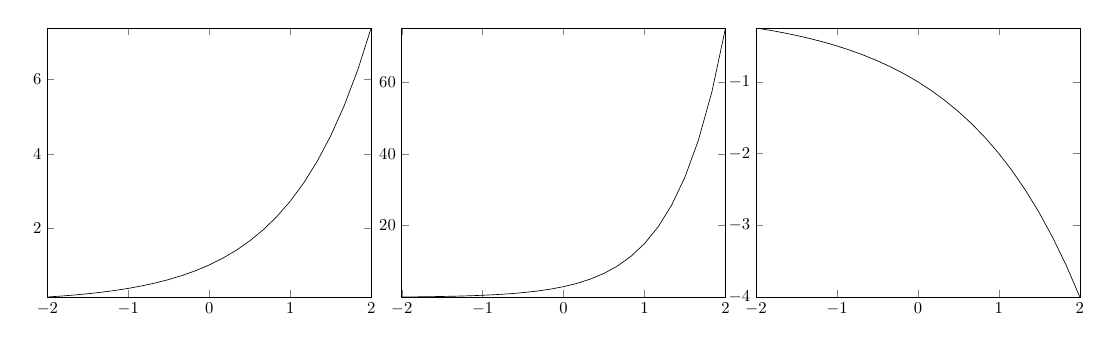
\begin{tikzpicture}
		\begin{scope}[scale = 0.6, local bounding box=left, xshift=-6cm]
			\begin{axis}[enlargelimits=false]
				\addplot[domain = -2:2] {exp(x)};
			\end{axis}
		\end{scope}
		\begin{scope}[scale = 0.6, local bounding box=left, xshift=1.5cm]
			\begin{axis}[enlargelimits=false]
				\addplot[domain = -2:2] {3*5^x};
			\end{axis}
		\end{scope}
		\begin{scope}[scale = 0.6, local bounding box=left, xshift=9cm]
			\begin{axis}[enlargelimits=false]
				\addplot[domain = -2:2] {-2^x};
			\end{axis}
		\end{scope}
	\end{tikzpicture}
	\caption{Illustration of examples $e^x$, $3(5^x)$, and $-2^x$ respectively with domain $[-2, 2]$. }
	\label{fig1}
\end{figure}
\par

In the function $y=ab^x$, $b^x$ represents an exponential function $a$ is regarded as a scaling factor. The function contains a single term and also can not be simplified or reduced to an alternate form. Some examples are show in figure \ref{fig1} and \ref{fig2} below. 
\par
The range of $y$ varies depending on various parameter as follows.
\begin{itemize}
	\item When $a<0$, $y\in(-\infty, 0)$.
	\item When $a>0$, $y\in(0, +\infty)$.
	\item When $a=0$, $y=0$, if $b=1$ then $y=a$.
	\item When $b=e$, $a=1$, $y=e^x$ (The exponential function. $y\in(0, +\infty)$).
\end{itemize}


\begin{figure}[H]
	\centering
	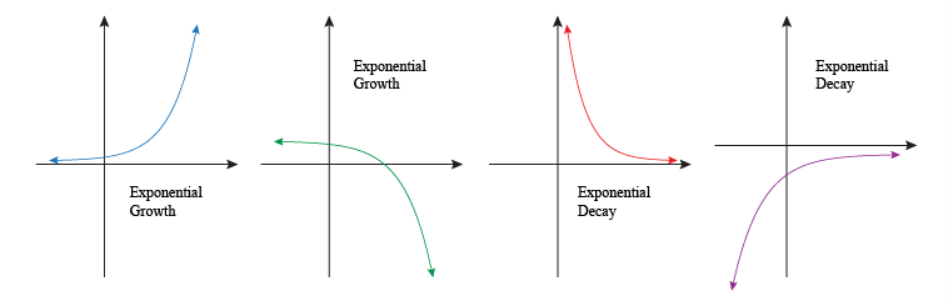
\includegraphics[width=\linewidth]{Figures/graph}
	\caption{Typical variations of $y=ab^x$ for standard trends.}
	\label{fig2}
\end{figure}

\subsection{Context of use model}
The calculator application as described by the function can accommodate two types of user namely. Scientists (human users) and external programs through Application Program Interface (API) calls on subordinate functions.\par
The main function takes as input valid double data types for the three parameters $a$, $b$ and $x$. These values are entered by the user through the user interface and validated by the program and then passed into the main method. This method in turn calls subordinate functions to obtain the relevant results. The calculator then return the final results of calculation to the user interface. This could be a value or simply a message indicating a calculation error. This process is illustrated in figure \ref{fig3} below \cite{contextofuse}.
\begin{figure}[H]
	\centering
	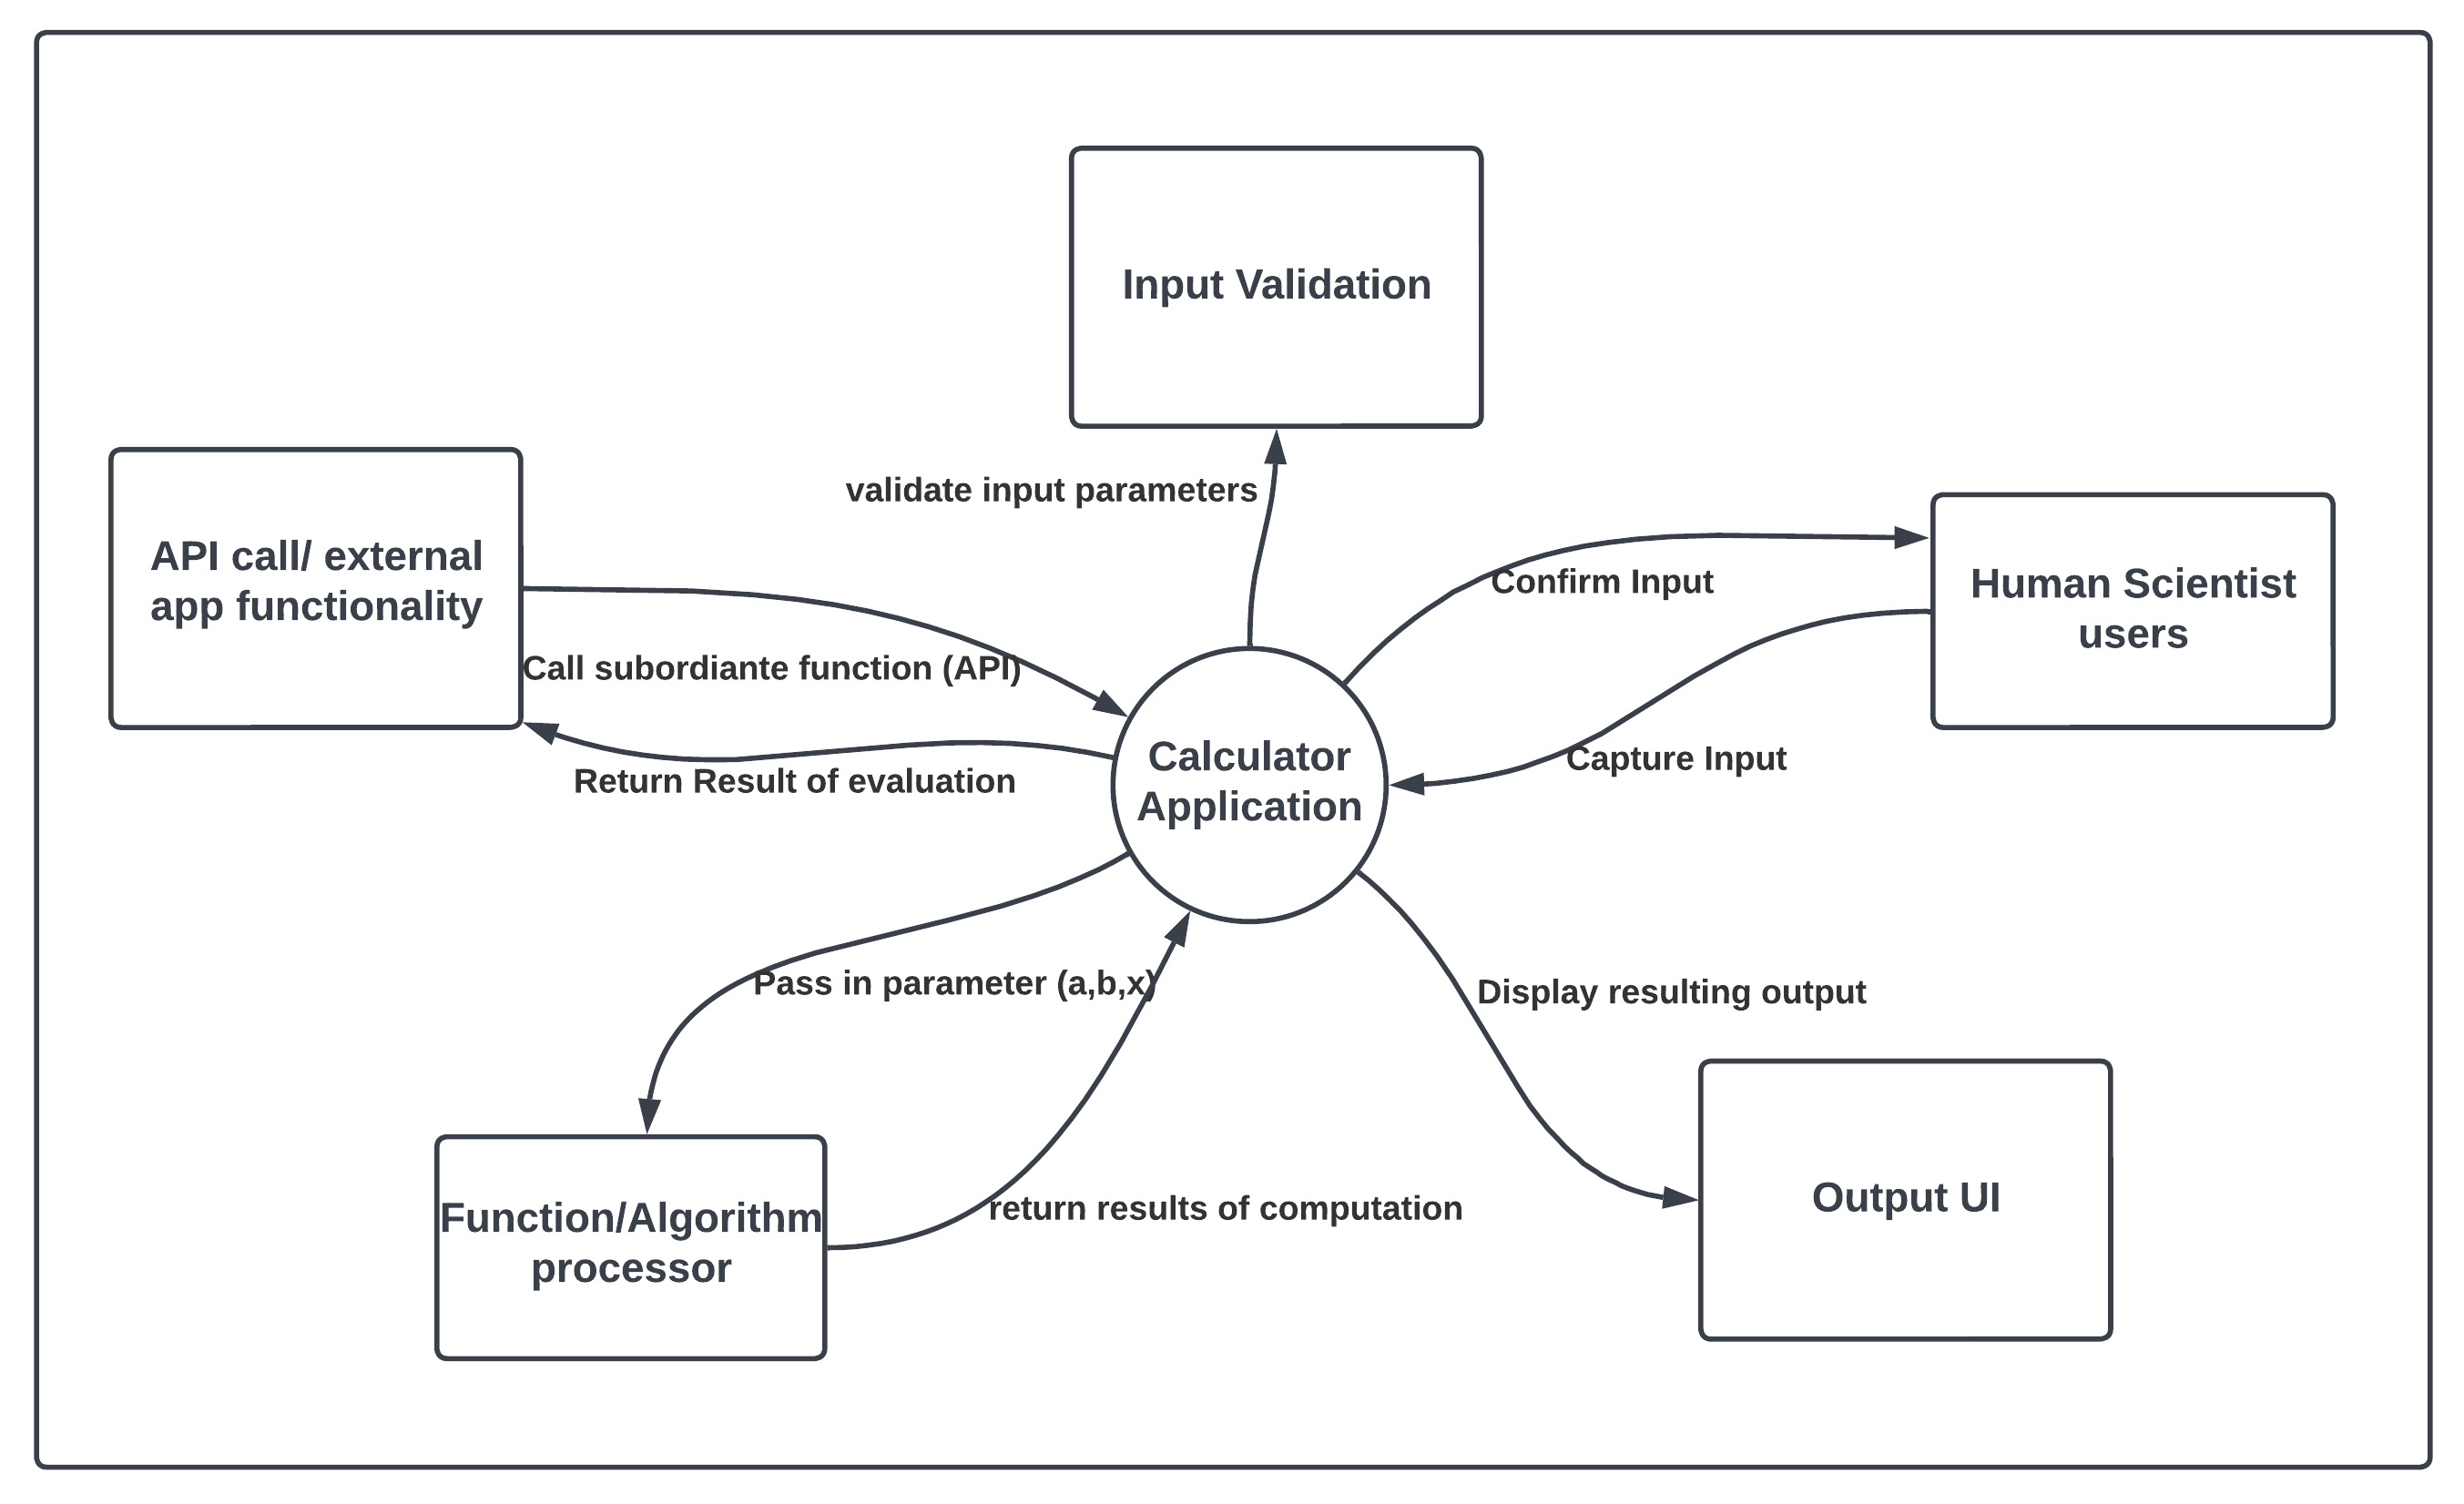
\includegraphics[width=\linewidth]{Figures/ContextDiagram}
	\caption{Context of use model for the program $y=ab^x$.}
	\label{fig3}
\end{figure}

\section{Requirement Extraction} \label{s:sec2}
In order to obtain a artefact through the software development process, it is necessary to formulate requirement of the system. These artefacts are usually the by-product produced during the development process (DevOps) include relevant designs diagrams and models use as described in the document \cite{ravid2000method}. We shall consider four main activities in the requirement extraction process as follows.
\subsection{Requirements elicitation}
At this stage we communicated intensively with stakeholders. In this case this was done by reading project description, clarifying requirements with the lecturer and discussing the assignment with teaching assistant and other fellow student to have more insights on the problem. The various approaches to the implementation of subordinate function were investigated and constraint were defined. The context diagram was developed and the necessary literature was conducted for various implementation. The users include human users and APIs. Mathematical concepts and implications were considered and there was revision of boundaries and constraints of the function $y=ab^x$. A draft of the UI design was discussed too with stakeholders. At this stage there is a clear understanding of the problem.
\subsection{Requirements specification}
Here we elaborate requirements formally based on the previous stage of the process. All requirements including functional and non-functional requirements, and constraints are specifies here \cite{li2015automated}. As studied in agile methodologies, these activities are carried out incrementally and iteratively as we develop the program by revising requirements. Git and GitHub was used as the version control system throughout the development process. 
\subsubsection{Functional requirements}
\begin{itemize}
	\item The program must be implemented in Java and the document written in Latex.
	\item The mathematical expressions in must be typeset in Latex and not as images.
	\item The artifacts must be placed in a distributed version control system.
	\item The algorithms must handle every boundary conditions of the domain and codomain of the function. 
	\item The main function ($y=ab^x$) and its subordinate functions ($e^x$, $a^x$, $\ln x$, $\lvert x \rvert$) must be implemented from scratch.
	\item Unit tests (JUnits) must be created to test each corresponding subordinate functions. This is done to test that our solution corresponds to or at least nearly equates to the actual value.
	\item A variable parameter $\epsilon$ may be provided by the user to control the allowable error in the calculations. A default value is used if $\epsilon$ is not provided.
\end{itemize}
\subsubsection{Non-functional requirements}
\begin{itemize}
	\item The program must be user friendly and well documented using software engineering best practices.
	\item The solution implementation must be scalable for various mathematical calculations and maintainable over time.
	\item The program must be portable. The algorithms and source code for the program and document (Latex) must run on any integrated development environment for the specified language (Java).
	\item The algorithms for subordinate functions must be designed to attain high performance in terms of both space and time complexities.
\end{itemize}
\subsection{Requirements verification and validation}
Verification is conducted to ensure the software implements the specific function. This is done by testing the implementation against a range of values and comparing them with the actual answers of default calculations.\par
Validations is carried out to ensure that the software matches various constraints and is traceable to customer requirements. This also help to avoid propagation of errors to successive stages. Unit test were developed for various constraint to satisfy the requirements of the function.
\subsection{Requirements management}
At this stage, we analyse, document, track, prioritise and agree on requirement while controlling communication with stakeholders. This is done through flash reviews organised by the lecturer to monitor progress thus far and make changes or validate requirements. We also produce relevant documentations and review on the implementation of the software.

\section{Source code review and description of test cases} \label{s:sec3}
The source code of the program conforms to google coding style and the variable names comply to the camel case standard nomenclature \cite{google2}. The code also aligns with the standard programming style for Java. Throughout the program exception handling, error messages and other error handling mechanisms are used to make the program robust, it also contribute to enforcing the constraints of the mathematical expressions. A graphical user interface is used to capture user inputs and display the program output. Google's code review guidelines was use to review the implementation of the function \cite{google1}.\par

\subsection{Pseudocode and description of Algorithms}
\begin{algorithm}[H]
	\caption{Algorithm for power($x$, $n$)}\label{alg:pow}
	\begin{algorithmic}
		\Require $n \geq 0$
		\Ensure $y = x^n$
		\State $y \gets 1$
		\State $X \gets x$
		\State $N \gets n$
		\While{$N \neq 0$}
		\If{$N$ is even}
		\State $X \gets X \times X$
		\State $N \gets \frac{N}{2}$  \Comment{setting $N$ to its half}
		\ElsIf{$N$ is odd}
		\State $y \gets y \times X$
		\State $N \gets N - 1$
		\EndIf
		\EndWhile
	\end{algorithmic}
\end{algorithm}

\begin{algorithm}[H]
	\caption{Algorithm for $\ln x$}\label{alg:ln}
	\begin{algorithmic}
		\Require $x > 0$, $nterms$
		\Ensure $y = \ln x$
		\State $result \gets 0.0$
		\While{$x > 2$}
			\State $result \gets result + \ln 2$
			\State $x \gets x/2$
		\EndWhile
		\State $x \gets x -1$
		\State $factor \gets 1$
		\State $res \gets 0.0$
		\For{$i \gets 1$ to $nterms$}
		\State $res \gets res + factor * power(x, i)/i$ \Comment{External call to Algorithm \ref{alg:pow}}
		\State $factor \gets factor - factor$
		\EndFor
		\State $result\gets result + res$
	\end{algorithmic}
\end{algorithm}

\begin{algorithm}[H]
	\caption{Algorithm for $e^x$}\label{alg:ex}
	\begin{algorithmic}
		\Require $x \in \mathbb{R}$, $nterms$ (Number of terms)
		\Ensure $y = e^x$
		\State $temp \gets 1$
		\State $result \gets 1.0$
		\For{$i \gets 1$ to $nterms$}\Comment{Taylor's Series Expansion of $\ln x$}
		\State $temp \gets temp * i$
		\State $result \gets results + power(x, i) / temp$
		\EndFor
	\end{algorithmic}
\end{algorithm}

\begin{algorithm}[H]
	\caption{Algorithm for $\lvert x \rvert$}\label{alg:abs}
	\begin{algorithmic}
		\Require $x \in \mathbb{R}$
		\Ensure $y = \lvert x \rvert$
		\If{$x$ is negative}
		\State $x \gets -x$
		\EndIf
	\end{algorithmic}
\end{algorithm}

\begin{algorithm}[H]
	\caption{Algorithm for $ab^x$}\label{alg:abx}
	\begin{algorithmic}
		\Require $x \in \mathbb{R}$, $a$, $x$
		\Ensure $y=ab^x$
		\State $result \gets a *power(b,x)$ \Comment{External call to Algorithm \ref{alg:pow}}	
	\end{algorithmic}
\end{algorithm}

\subsection{Test cases and tool used}
The program is implemented using Eclipse IDE for developers (version 2021-09) \cite{eclipse}. The program is illustrated below. The Latex code was written in TeXstudio (version 4.0.0). Java Developer Tools (JDT) such as JUnit (JUnit 5 for Eclipse Oxygen was used) to build test cases. The coverage was computed with JaCoCo library, a plug-in in Eclipse.
\begin{figure}[H]
	\centering
	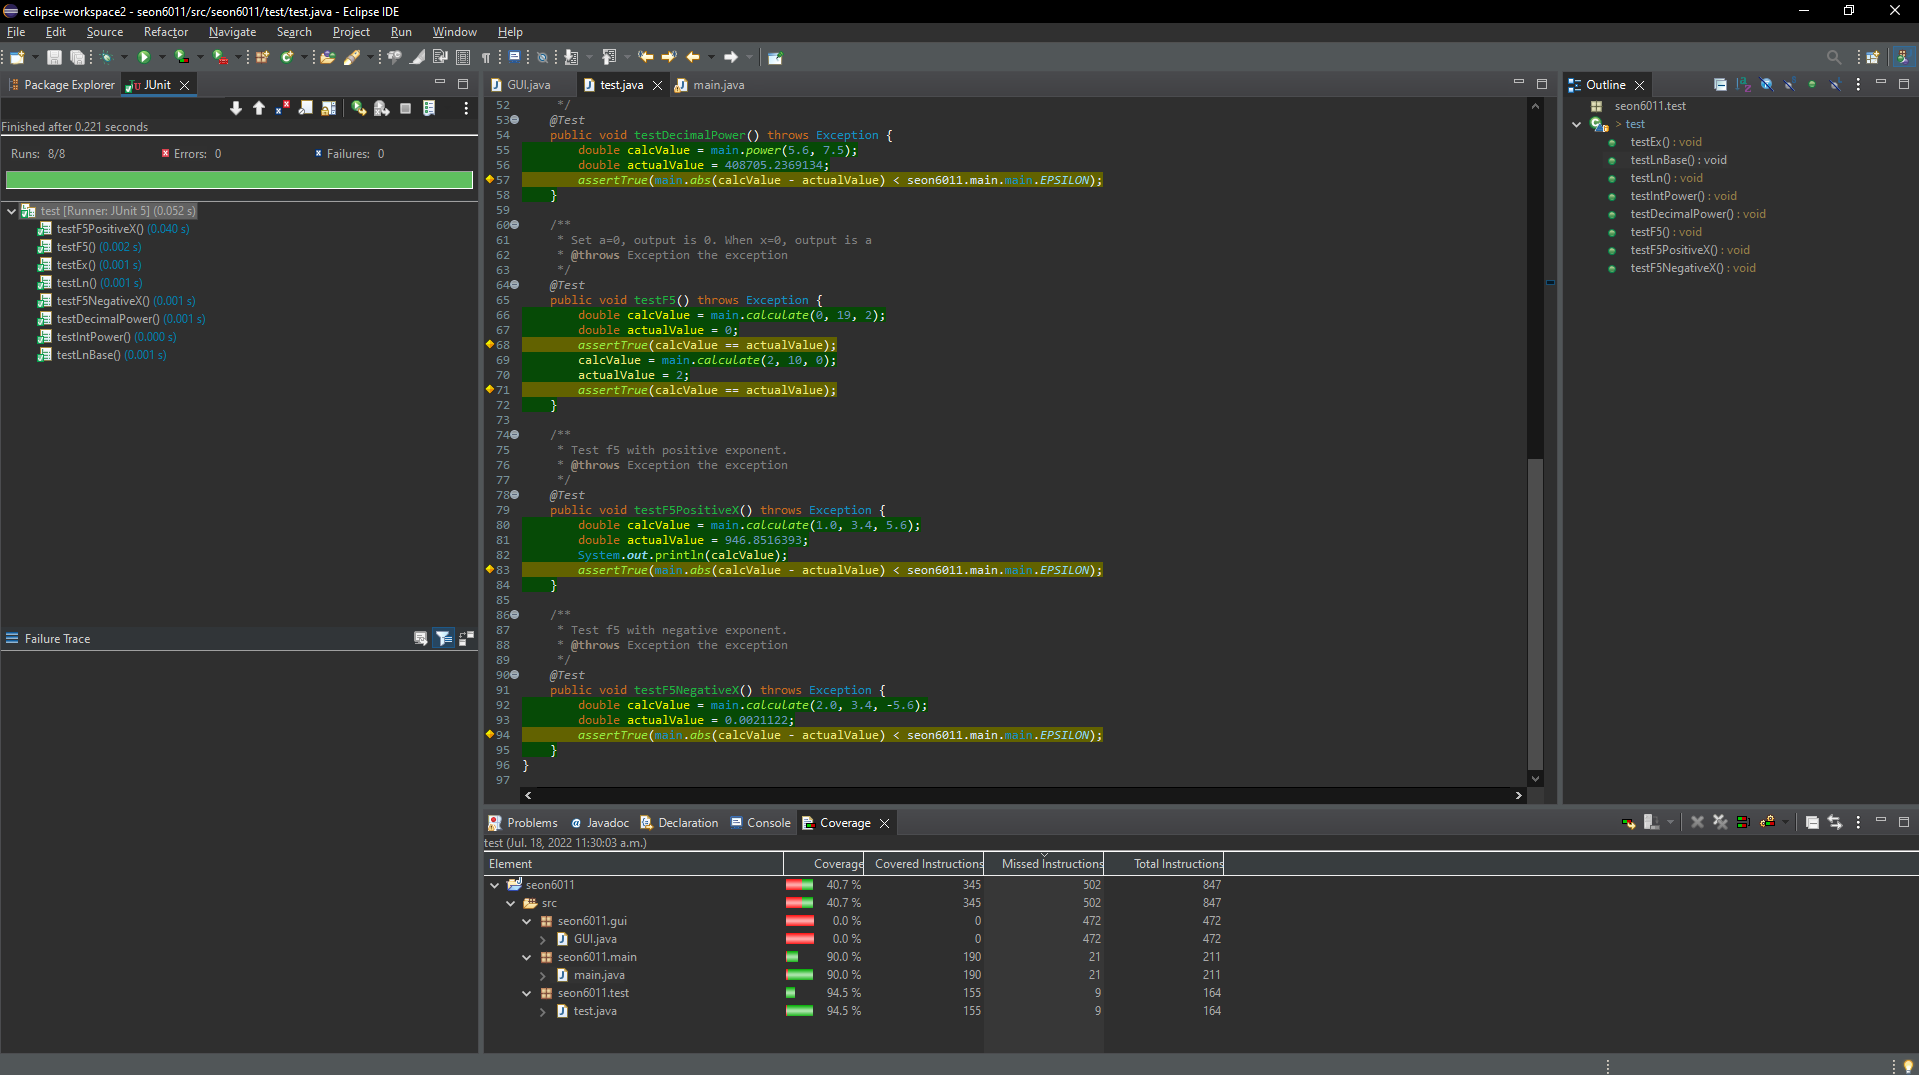
\includegraphics[width=\linewidth]{Figures/test}
	\caption{Test cases showed in the debugger.}
	\label{fig4}
\end{figure}
\par Both the Javadoc and test case coverage was exported and stored in the source folder of the program. The graphical user interface was implemented with the \emph{javax.swing} library.

\subsubsection{Advantages of Eclipse}
\begin{itemize}
	\item Eclipse is a free and open source IDE which supports multiple languages and is a especially suited for Java, it is one of the most popular IDEs for Java.
	\item It supports a wide range of plug-ins, allowing users to make their own plug-in development environment (PDE).
	\item Eclipse provides modelling support for projects including Unified Modelling Language (UML).
\end{itemize}
\subsubsection{Disadvantages of Eclipse}
\begin{itemize}
	\item Eclipse tends to be significantly slow to run compared with other IDEs such as NetBeans due to insufficient memory allocation.
\end{itemize}

\begin{figure}[H]
	\centering
	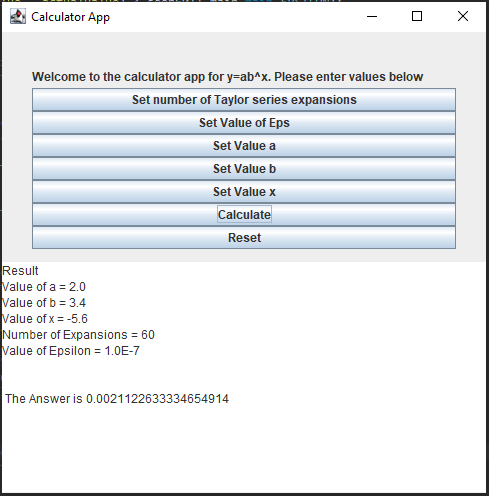
\includegraphics[width=0.7\linewidth]{Figures/gui}
	\caption{Graphical user interface for Calculator App $y=ab^x$.}
	\label{fig5}
\end{figure}

\section{Conclusion}\label{s:conclusion}
In conclusion, we described, implemented and documented the scientific calculation of the function $y=ab^x$ using software engineering best practices. The program was built conceptually and tested in Java programming language, we designed a also designed a context of use that fits with the implementation.


\bibliographystyle{abbrv}
\spacingset{1}
\bibliography{References}
	
\end{document}
